\section{Gruppenantennen}\label{sec:gruppenantennen}
Der Dipol ist ein Rundstrahler, da die Strahlung keine bevorzugte Richtung in der Ebene senkrecht zur Antennenachse aufweist. Bei Punkt-zu-Punkt Verbindungen kann die Reichweite der Antenne bei unveränderter Energie erheblich vergrössert werden, wenn eine Richtwirkung vorhanden ist. Mit der Richtwirkung lässt sich der Störabstand verbessern, da mögliche Störquellen durch die Richtcharakteristik zum Teil ausgeblendet werden. Eine gewünschte Richtwirkung kann durch Kombination zweier oder mehrerer Dipole mittels Interferenz der Feldstärken erzeugt werden. 

Die folgenden Betrachtungen basieren auf dem linearen Superpositionsprinzip. Dies geht davon einer ungestörten Überlagerung der Strahlungsbeiträge aller Teilstrahler aus. Das Maximum des resultierenden Feldes befindet sich dort, wo die Felder der Einzelstrahler phasengleich schwingen. Die Felder der Einzelstrahler die ausserhalb der Hauptstrahlungsrichtung sind, löschen sich gegenseitig mehr oder weniger aus. Die Richtwirkung kann mit diesen Faktoren beeinflusst werden.

\begin{itemize}
	\item Anzahl Strahler
	\item Anordnung der Strahler
	\item Stromamplitude der einzelnen Strahler
	\item Phasenverschiebung der einzelnen Strahler
\end{itemize}

In der Abbildung \ref{fig:gruppenantennen} sind drei unterschiedliche Formen von Gruppen aus Dipolantennen die sich für die Nachrichtenübertragung bewährt haben. 

\begin{figure}[H]
	\centering
	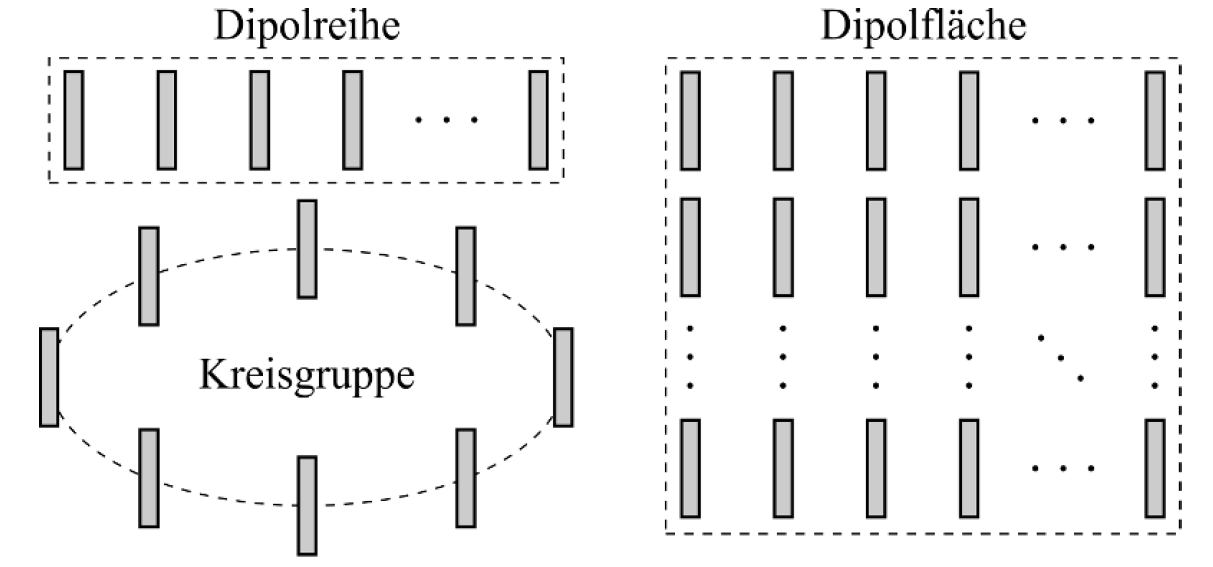
\includegraphics[width=0.75\linewidth]{gruppenantennen}
	\caption{Anordnung von Einzelstrahlern zu einer Antennengruppe}\label{fig:gruppenantennen}
\end{figure}


\subsection{Querstrahler}\label{sec:querstrahler}

Der Querstrahler gehört zu den linearen Gruppenstrahler und ist eine Dipolzeile. In der 

\begin{figure}[H]
	\centering
	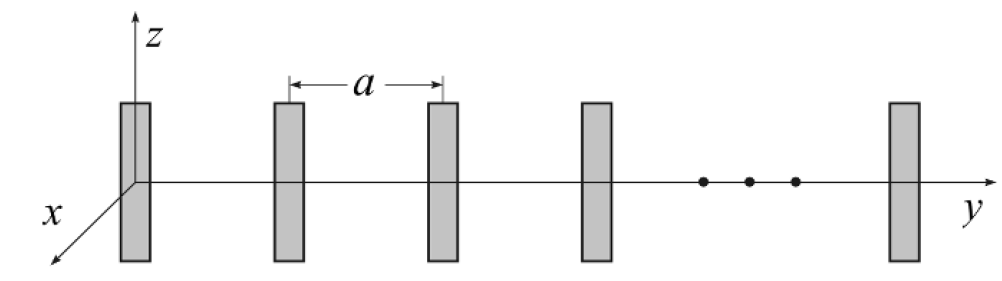
\includegraphics[width=0.75\linewidth]{dipolzeile}
	\caption{Anordnung von baugleichen, äquidistanten Einzelstrahlern zu einer Horizontaler Dipolzeile }\label{fig:dipolzeile}
\end{figure}